%-------------------------
% Resume in Latex
% Author : David
% Based on: https://github.com/jakegut/resume (which was based on https://github.com/sb2nov/resume)
% License : MIT
%------------------------

\documentclass[letterpaper,11pt]{article}

\usepackage{latexsym}
\usepackage[empty]{fullpage}
\usepackage{titlesec}
\usepackage{marvosym}
\usepackage[usenames,dvipsnames]{color}
\usepackage{verbatim}
\usepackage{enumitem}
\usepackage{fancyhdr}
\usepackage[english]{babel}
\usepackage{tabularx}
\usepackage{xcolor}
\usepackage{fontawesome5}
\usepackage{graphicx}

\input{glyphtounicode}

% -------------------- FONT --------------------
\pagestyle{fancy}
\fancyhf{} % clear all header and footer fields
\fancyfoot{}
\renewcommand{\headrulewidth}{0pt}
\renewcommand{\footrulewidth}{0pt}

% Adjust margins
\addtolength{\oddsidemargin}{-0.5in}
\addtolength{\evensidemargin}{-0.5in}
\addtolength{\textwidth}{1in}
\addtolength{\topmargin}{-1in} % Default was -.5in
\addtolength{\textheight}{1.0in}

\urlstyle{same}

\raggedbottom
\raggedright
\setlength{\tabcolsep}{0in}

% Section formatting
\titleformat{\section}{
  \vspace{-5pt}\scshape\raggedright\large
}{}{0em}{}[\color{black}\titlerule \vspace{-5pt}]

% Subsection formatting
\titleformat{\subsection}{
  \vspace{-4pt}\scshape\raggedright\large
}{\hspace{-.15in}}{0em}{}[\color{black}\vspace{-8pt}]

% Ensure that generate pdf is machine readable/ATS parsable
\pdfgentounicode=1

% -------------------- CUSTOM COMMANDS --------------------
\newcommand{\resumeItem}[1]{
  \item\small{
    {#1 \vspace{-2pt}}
  }
}

\newcommand{\resumeSubheading}[4]{
  \vspace{-2pt}\item
    \begin{tabular*}{0.97\textwidth}[t]{l@{\extracolsep{\fill}}r}
      \textbf{#1} & #2 \\
      \textit{\small#3} & \textit{\small #4} \\
    \end{tabular*}\vspace{-7pt}
}

\newcommand{\resumeSubSubheading}[2]{
    \item
    \begin{tabular*}{0.97\textwidth}{l@{\extracolsep{\fill}}r}
      \textit{\small#1} & \textit{\small #2} \\
    \end{tabular*}\vspace{-7pt}
}

\newcommand{\resumeProjectHeading}[2]{
    \item
    \begin{tabular*}{0.97\textwidth}{l@{\extracolsep{\fill}}r}
      \small#1 & #2 \\
    \end{tabular*}\vspace{-7pt}
}

\newcommand{\resumeSubItem}[1]{\resumeItem{#1}\vspace{-4pt}}
\newcommand{\resumeSubHeadingListStart}{\begin{itemize}[leftmargin=0.15in, label={}]}
\newcommand{\resumeSubHeadingListEnd}{\end{itemize}}
\newcommand{\resumeItemListStart}{\begin{itemize}}
\newcommand{\resumeItemListEnd}{\end{itemize}\vspace{-5pt}}

\renewcommand\labelitemii{$\vcenter{\hbox{\boldmath$\cdot$}}$}
\renewcommand\labelitemi{{\boldmath$\cdot$}}

\setlength{\footskip}{4.08003pt}

% -------------------- START OF DOCUMENT --------------------
\begin{document}

% -------------------- HEADING--------------------
% \begin{flushright}
%     \vspace{-4pt}
%     \color{gray}
%     \item
%     % Last Updated on September 9th, 2023
% \end{flushright}


\begin{minipage}{.95\linewidth}
\vspace{25pt}
\begin{center}
    \textbf{\Huge \scshape David Petri} \\ \vspace{8pt}
    \small
    \faIcon{github}
    {github.com/dapetri} $  $
    \faIcon{code}
    {dapetri.com} $  $
    \faIcon{linkedin}
    {linkedin.com/in/dapetri} $  $
    \faIcon{envelope}
    {me@dapetri.com} $  $ \\
    \faIcon{home}
    {Hans-Thoma-Str. 47, 69121 Heidelberg (DE)} $  $
    \faIcon{phone}
    {+49 173 7777637} $  $
\end{center}
\end{minipage}\hfill

\begin{picture}(0,0)
    \put(460,-9){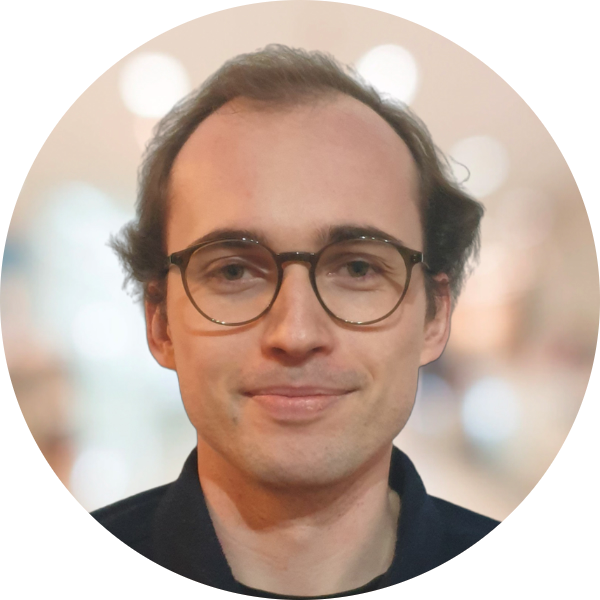
\includegraphics[width=6.5em]{img/profile-pic-2.png}}
\end{picture}

\vspace{-8pt}
% 
% -------------------- EXPERIENCE --------------------
\section{Experience}
\resumeSubHeadingListStart

\resumeProjectHeading
{\textbf{Machine Learning Engineer Intern} $|$ \footnotesize\emph{BMW Group - Munich (DE)}\vspace{8pt}}{Nov. 2023 -- \textit{present}}
{\small{Python, PyTorch Lightning, OpenCV, Supervisely, AIQX, Anomalib, Git}}
\vspace*{-5pt}
\resumeItemListStart
\resumeItem{Development and implementation of a \textbf{data preprocessing pipeline} for a \textbf{first-of-a-kind industrial labeled dataset}.}
\resumeItem{Development and training of an \textbf{Anomaly Detection Deep Convolutional Neural Network} for the visual identification of production errors in V8 and V12 engines.}
\resumeItemListEnd

\vspace{5pt}
\resumeProjectHeading
{\textbf{Machine Learning Researcher} $|$ \footnotesize\emph{Karlsruhe Institute of Technology - Karlsruhe (DE)}\vspace{8pt}}{Apr. 2023 -- Nov. 2023}
{\small{Python, PyTorch (Geometric), NumPy, SciPy, Matplotlib, Git}}
\vspace*{-5pt}
\resumeItemListStart
\resumeItem{Learned an \textbf{Adaptive Mesh Refinement} strategy for the \textbf{Finite Element Method} through expert demonstrations and preferences by using \textbf{Generative Adversarial Imitation Learning} to train the \textbf{Proximal Policy Optimization} \textbf{Reinforcement Learning} algorithm.}
\resumeItem{Achieved a \textbf{91\% coverage} with the expert strategy distribution.}
\resumeItemListEnd

\vspace{5pt}
\resumeProjectHeading
{\textbf{Machine Learning Researcher Intern} $|$ \footnotesize\emph{Karlsruhe Institute of Technology}\vspace{8pt}}{Oct. 2021 -- Apr. 2022}
{\small Python, PyTorch (Vision), OpenCV, Open3D, NumPy, Git}
\vspace*{-5pt}
\resumeItemListStart
\resumeItem{Developed and implemented a \textbf{data preprocessing pipeline} to \textbf{record, transform} and \textbf{mask 3D images}.}
\resumeItem{Trained a \textbf{Deep Convolutional Neural Network} for \textbf{denoising depth-maps of 3D images}.}
\resumeItem{Achieved a \textbf{60\% reduction of noise} in the depth images.}
\resumeItemListEnd

\vspace{5pt}
\resumeProjectHeading
{\textbf{Software Developer Freelance} $|$ \footnotesize\emph{Kuori Materials, Basel (CH)}\space [kuori.ch]\vspace{8pt}}{May 2021 -- Aug. 2021}
{\small TypeScript, React, HTML/CSS, Node.js, Git}
\vspace*{-5pt}
\resumeItemListStart
\resumeItem{Developed the company's ebsite according to specifications of the design department.}
\resumeItem{Successfully \textbf{deployed} and \textbf{maintained} the \textbf{first internet presence} of the company.}
\resumeItemListEnd

\resumeSubHeadingListEnd
% -------------------- EDUCATION --------------------
\section{Education}
\resumeSubHeadingListStart

\resumeSubheading
{Master of Science in Computer Science}{2021 - 2023}
{Karlsruhe Institute of Technology (DE)}{GPA: \textbf{top 10\%} - DE \textbf{1.4}, US 3.8/4.0, CH 5.6/6.0}

\vspace{3pt}

\resumeSubheading
{Bachelor of Science in Computer Science}{2018 - 2021}
{Karlsruhe Institute of Technology (DE)}{GPA: DE 2.0, US 3.5/4.0, CH 5.0/6.0}

\vspace{3pt}

\resumeSubheading
{Bachelor of Science in Business \& Economics}{2015 - 2018}
{Johannes Gutenberg University Mainz (DE) /}{GPA: DE 1.9, US 3.55/4.0, CH 5.1/6.0}

\vspace{2pt}
\textit{\small Ca'Foscari University of Venice (IT)}

\vspace{2pt}
\begin{tabular*}{0.7\textwidth}{@{\hskip 0.1in}l@{\hskip 0.1in}l}
    {\small \textbf{\textit{Coursework:}}} & {\small Machine Learning, Deep Learning, Neural Networks, Computer Vision, Distributed \& Scalable AI,} \\
    {\space} & {\small Mathematics, Statistics, Optimization Methods, Reinforcement Learning, Robotics, Telematics}
\end{tabular*}\vspace{-7pt}



\resumeSubHeadingListEnd

  
% -------------------- publications --------------------
\section{Publications}
\resumeItemListStart
\resumeItem{\textbf{Learning Adaptive Mesh Refinement Strategies from Human Feedback} [Freymuth, Petri et al., \textit{in prep.}]}
\vspace*{-5pt}
\resumeItem{\textbf{Multi-Object Self-Supervised Depth Denoising} [Kienle \& Petri, 2023, arXiv: 2305.05778]}
\resumeItemListEnd
\vspace*{-7pt}

% -------------------- skills --------------------
\section{Skills}
\begin{itemize}[leftmargin=0.15in, label={}]
    \small{\item{
                    \begin{tabbing}
                        \textbf{Pragramming Languages} ~~~ \={Python (4 Y.), Java (2 Y.), R (2 Y.), SQL (4 Y.), Java-/TypeScript} \\
                        \textbf{Libraries} \> {PyTorch (3 Y.), OpenCV, Open3D, NumPy, SciPy, Pandas, Matplotlib} \\
                        \textbf{Tools/Frameworks} \> {Git (4 Y.), Docker (2 Y.), React (2 Y.)} \\
                        \textbf{Spoken Languages} \> {German: \textit{native},\quad English: \textit{C2} - TOEFL 114/120},\ \\ \> Italian: \textit{B2},\quad \quad \quad  Spanish: \textit{B1},\quad French: \textit{DELF B1},\quad Hungarian: \textit{A2}

                        % \textbf{Certificates} \> {AWS Certified Cloud Practitioner}


                    \end{tabbing}
                }}
\end{itemize}

% -------------------- PROJECTS --------------------
\vspace{-10pt}
\section{Hobbies}
\begin{tabular}{ l l l}
    
    \quad \small · Chess:  Elo $\sim$ 1550 \quad \quad \quad &\small \quad · Learning new languages \quad \quad · \small Play Basketball \quad \quad · Refurbishing Old-Timer Motorbikes 
    % \quad · \small Basketball &\small \quad · Refurbishing Old-Timer Motorbikes \\  
\end{tabular}

\end{document}
